\documentclass[UTF8,a4paper]{ctexart}

% ==========Preamble==========
\usepackage{graphicx}
\usepackage{listings}
\usepackage{apacite}
\usepackage{url}
\usepackage{fancyhdr}
\usepackage{geometry}
\usepackage[font=small,labelfont=bf,labelsep=quad,format=hang,textfont=it]{caption}
\usepackage{booktabs}
\usepackage{graphicx}
\usepackage{float}
\usepackage{xcolor}
\usepackage{amsmath}
\DeclareMathOperator{\sign}{sign}

\definecolor{commentcolor}{RGB}{85,139,78}
\definecolor{stringcolor}{RGB}{206,145,108}
\definecolor{keywordcolor}{RGB}{34,34,250}
\definecolor{backcolor}{RGB}{220,220,220}

\pagestyle{plain}
\CTEXsetup[format=\Large\bfseries]{section}
\bibliographystyle{apacite}
\DeclareGraphicsExtensions{.eps,.pdf,.jpg,.png}

%设置代码
\lstset{
	%backgroundcolor=\color{red!50!green!50!blue!50},%代码块背景色为浅灰色
%	rulesepcolor= \color{gray}, %代码块边框颜色
    commentstyle=\color{commentcolor},	%注释颜色
	keywordstyle=\color{keywordcolor},	%关键词颜色
	stringstyle=\color{stringcolor},	%字符串颜色
	breaklines=true,  %代码过长则换行
	numbers=left, %行号在左侧显示
	numberstyle= \small,%行号字体
	%keywordstyle= \color{blue},%关键字颜色
	commentstyle=\color{gray}, %注释颜色
%	frame=shadowbox%用方框框住代码块
	frame=single,
	escapeinside=``    % 代码包含中文
}

% 设置图表搜索路径, 可以给图表文件夹取如下名字
\graphicspath{{img/}}

% ==========Title==========

\title{\bfseries 第三章作业 } 
\author{\bfseries 谈昊\quad2020E8013282037}

% Your name in the first blank and your additional information in \thanks{}
\date{}
% delete \today if you don't want the date

% ==========Document==========

\begin{document}
\maketitle

\paragraph{Question}
\begin{itemize}
    \item[一、] 在一个10类的模式识别问题中,有3类单独满足多类情况1,其余的类别满足多类情况2。问该模式识别问题所需判别函数的最少数目是多少?
    \item[二、]
    一个三类问题,其判别函数如下:
    \begin{itemize}
        \item
    \begin{itemize}
        \item $d_1(x)=-x_1$
        \item $d_2(x)=x_1+x_2-1$
        \item $d_3(x)=x_1-x_2-1$
    \end{itemize}
    \item[(1)]设这些函数是在多类情况1条件下确定的,绘出其判别界面和每一个模式类别的区域。
    \item[(2)]设为多类情况2,并使:$d_{12}(x)= d_1(x), d_{13}(x)= d_2(x), d_{23}(x)= d_3(x)$。绘出其判别界面和多类情况2的区域。 
    \item[(3)]设$d_1(x)$, $d_2(x)$和$d_3(x)$是在多类情况3的条件下确定的,绘出其判别界面和每类的区域。
    \end{itemize}
    \item[三、] 两类模式,每类包括5个3维不同的模式向量,且良好分布。如果它们是线性可分的,问权向量至少需要几个系数分量?假如要建立二次的多项式判别函数,又至少需要几个系数分量?(设模式的良好分布不因模式变化而改变。)
    \item[四、] 用感知器算法求下列模式分类的解向量$w$:
        \begin{itemize}
            \item $\omega _1: {(0,0,0)^T, (1,0,0)^T, (1,0,1)^T, (1,1,0)^T}$
            \item $\omega _2: {(0,0,1)^T, (0,1,1)^T, (0,1,0)^T, (1,1,1)^T}$
        \end{itemize}
编写求解上述问题的感知器算法程序。


        
    \item[五、] 用多类感知器算法求下列模式的判别函数:
    \begin{itemize}
        \item $\omega _1: (-1 ,-1)^T$
        \item $\omega _2: (0, 0)^T$
        \item $\omega _3: (1 ,1)^T$
        
    \end{itemize}
    
    \item[六、] 编写求解上述问题的感知器算法程序,求下列模式分类的解向量w:
    \begin{itemize}
        \item $\omega _1: {(0 ,0 ,0)^T, (1 ,0 ,0)^T, (1 ,0 ,1)^T, (1 ,1 ,0)^T}$
        \item 
        $\omega _2: {(0 ,0 ,1)^T, (0 ,1, 1)^T, (0, 1 ,0)^T, (1 ,1 ,1)^T}$
    \end{itemize}
    尝试不同的初始值
    尝试不同的迭代顺序


\item[七、] 采用梯度法和准则函数
$$J(w, x, b)=\frac{1}{8\|x\|^{2}}\left[\left(w^{T} x-b\right)-\left|w^{T} x-b\right|\right]^{2}$$
式中实数b>0,试导出两类模式的分类算法。
\item[八、] 用二次埃尔米特多项式的势函数算法求解以下模式的分类问题
\begin{itemize}
    \item $\omega _1: {(0 ,1)^T, (0 ,-1)^T}$
    \item $\omega _2: {(1, 0)^T, (-1, 0)^T}$
\end{itemize}



\item[九、] 用下列势函数
$$
K\left(x, x_{k}\right)=e^{-\alpha\left\|x-x_{k}\right\|^{2}}
$$
	
求解以下模式的分类问题
\begin{itemize}
    \item $\omega _1: {(0 ,1)^T, (0 ,-1)^T}$
    \item $\omega _2: {(1, 0)^T, (-1, 0)^T}$
\end{itemize}
编写求解上述问题的感知器算法程序
\end{itemize}

\paragraph{Answer}
\begin{itemize}
    \item[一、] 多类情况1:$M$类需要$M$个判别函数,因此需要$3$个判别函数
    \\多类情况2:$M$类需要$M(M-1)/2$,因此需要$7*(7-1)/2 = 21$个判别函数
    \\因此共需要$3+21 = 24$个判别函数
    \item[二、] 
    \begin{itemize}
        \item[(1)] 如下图:
        \begin{figure}[H]
            \centering
            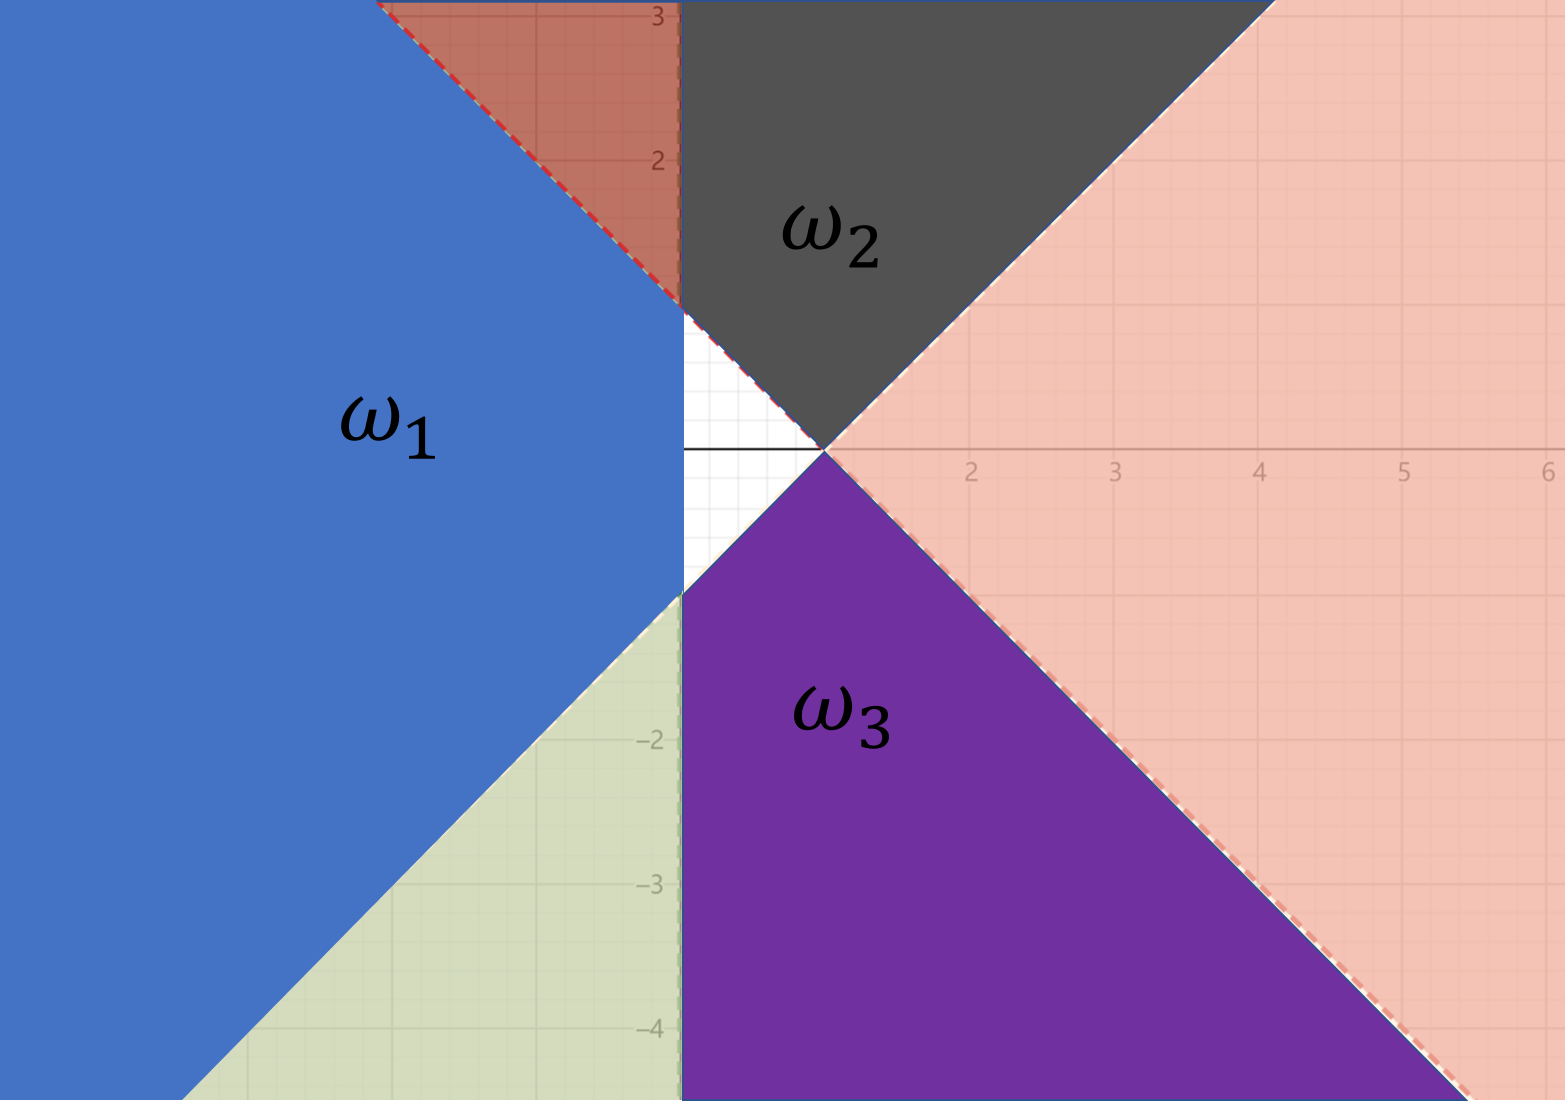
\includegraphics[width = 0.5\textwidth]{2-1.png}
            \end{figure}
        \item[(2)]如下图:
        \begin{figure}[H]
            \centering
            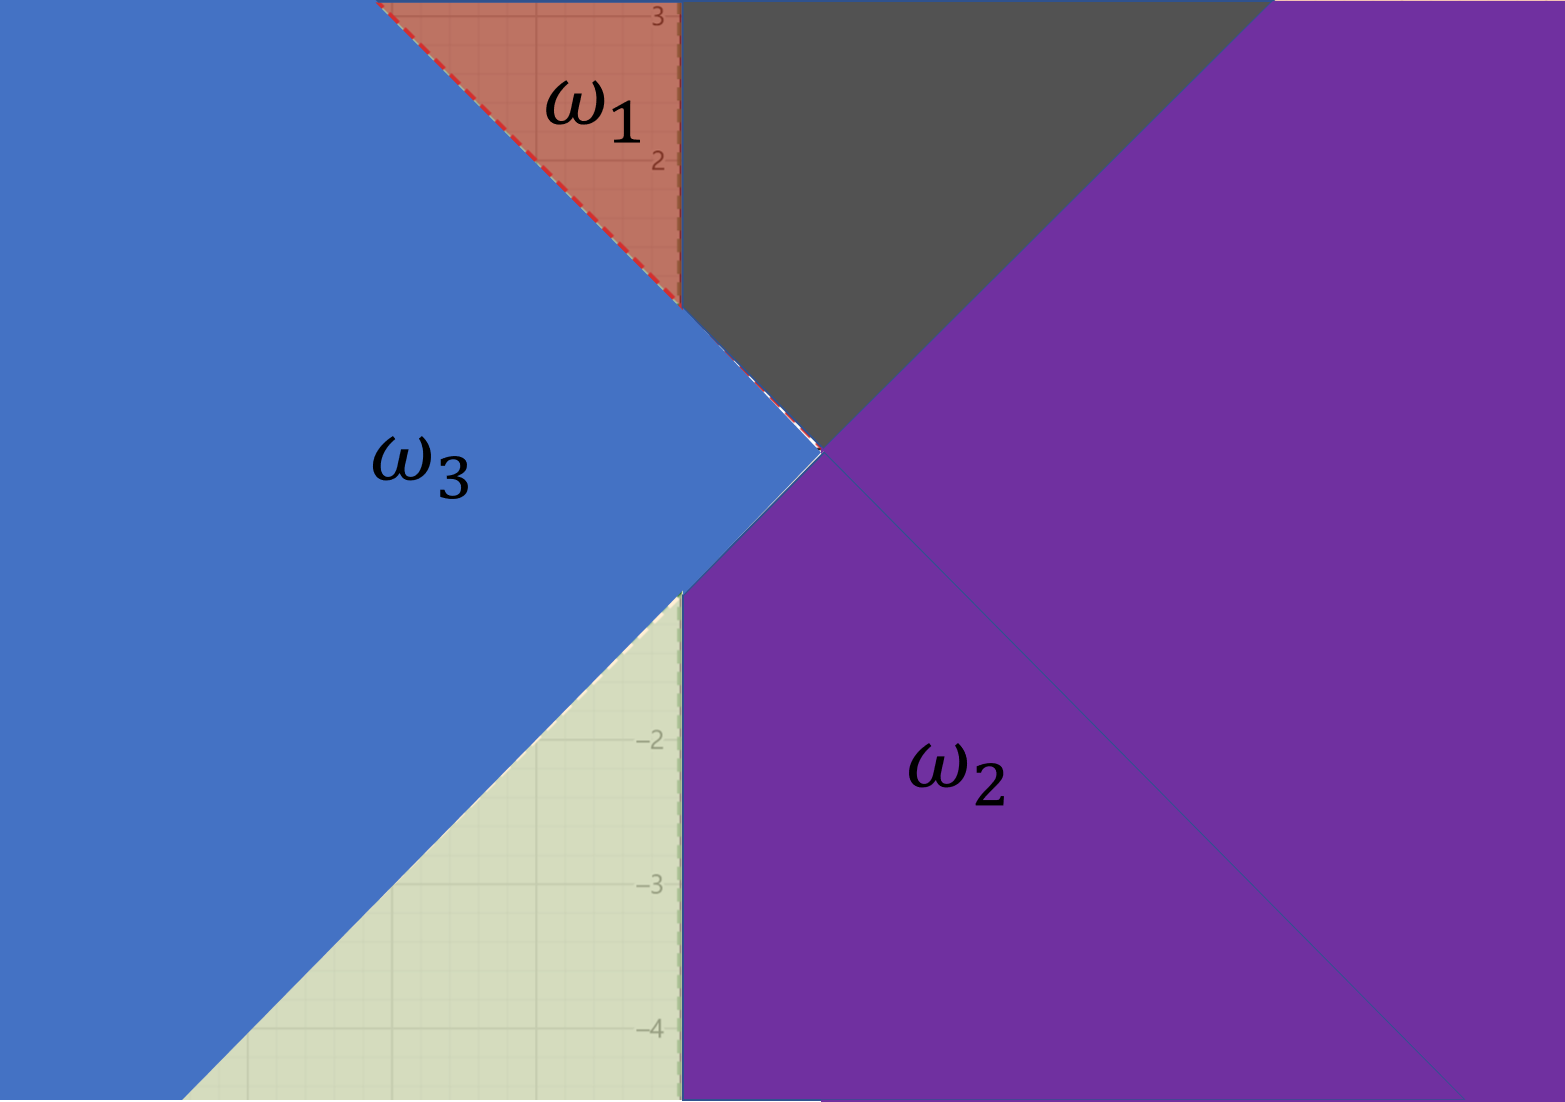
\includegraphics[width = 0.5\textwidth]{2-2.png}
            \end{figure}
        \item[(3)]如下图:
        \begin{figure}[H]
            \centering
            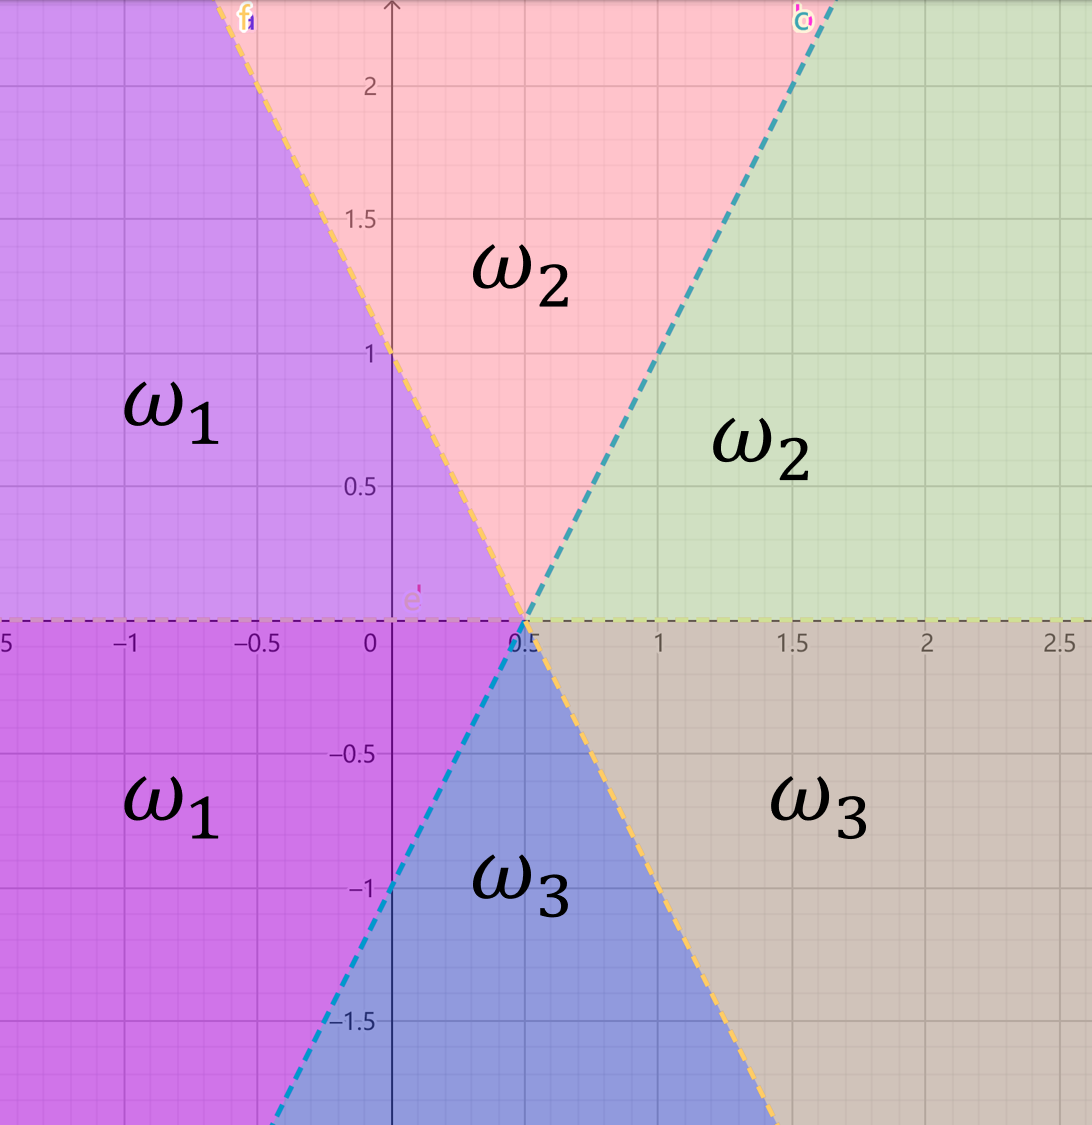
\includegraphics[width = 0.5\textwidth]{2-3.png}
            \end{figure}
    \end{itemize}

    \item[三、]
    根据公式$$\mathrm{N}_{\mathrm{w}}=\mathrm{C}_{\mathrm{n}+\mathrm{r}}^{\mathrm{r}}=\frac{(\mathrm{n}+\mathrm{r}) !}{\mathrm{r} ! \mathrm{n} !}$$
    因为线性可分,因此仅需$3$个权向量系数;若不可分,则需要$\frac{5!}{3!2!}=10$个权向量系数
\item[四、] 
\begin{itemize}
    \item 解向量$w$为:$(4,-3,-2)$
    \item 代码:\begin{lstlisting}[language={Python}]
        import numpy as np

        if __name__ == '__main__':
            w_1 = np.array([[0, 0, 0], [1, 0, 0], [1, 0, 1], [1, 1, 0]])
            w_2 = np.array([[0, 0, 1], [0, 1, 1], [0, 1, 0], [1, 1, 1]])
            c = 1
            w_2 *= -1
            w_all = np.vstack((w_1, w_2))
            w = np.array([0, 0, 0])
            flag = [-1] * (w_all.shape[0])
            i = 0
            while -1 in flag:
                i %= len(flag)
                x = w_all.data.obj[i]
                res = np.dot(x, w)
                if res > 0:
                    flag[i] = 0
                else:
                    w += x
                    flag[i] = -1
                i += 1
            print(w)
        
    \end{lstlisting}
\end{itemize}
\item[五、] 
\begin{itemize}
    \item 判别函数:$d_1(x) = -2x_1-2x_2-2x_3,d_2(x)=0,d_3(x)=2x_1+2x_2-2x_3$
    \item 代码为:
    \begin{lstlisting}[language={Python}]
import numpy as np


def mat_max_index(x, w):
    res = [np.dot(x, value) for value in w.data.obj]
    max_item = max(res)
    max_count = res.count(max_item)
    max_index = res.index(max(res)) if max_count == 1 else -1
    return max_index


if __name__ == '__main__':
    O = np.array([[-1, -1], [0, 0], [1, 1]])
    O = np.insert(O, O.shape[1], values=1, axis=1)

    W = np.array([[0, 0, 0], [0, 0, 0], [0, 0, 0]])

    flag = [-1] * O.shape[0]
    i = 0
    while -1 in flag:
        flag = [-1] * O.shape[0]
        for i, o in enumerate(O):
            if i == mat_max_index(o, W):
                flag[i] = 0
            else:
                for j, w in enumerate(W):
                    if j == i:
                        w += o
                    else:
                        w -= o
    print(W)
    \end{lstlisting}
\end{itemize}
\item[六、] 无变化,同四
\item[七、] 对准则函数求导可得
$$
\frac{\partial J}{\partial w}=\frac{1}{4\|x\|^{2}}\left[\left(w^{t} x-b\right)-\left|w^{t} x-b\right|\right] *\left[x-x* \operatorname{sgn}\left(w^{t} x-b\right)\right]
$$
其中,$$
\operatorname{sgn}\left(w^{t} x-b\right)=\left\{\begin{array}{c}
1, w^{t} x-b>0 \\
-1, w^{t} x-b \leq 0
\end{array}\right.
$$
得迭代式:$$
w(k+1)=w(k)+\frac{C}{4\|x\|^{2}}\left[\left(w(k)^{t} x-b\right)-\left|w(k)^{t} x-b\right|\right]*\left[x-x*\operatorname{sgn}\left(w(k)^{t} x-b\right)\right]
$$
故得$$
w(k+1)=w(k)+C\left\{\begin{array}{ll}
0 & w^{\prime} x-b>0 \\
\frac{\left(b-w^{t} x\right)}{\|x\|^{2}} x & w^{t} x-b \leq 0
\end{array}\right.
$$
\item[八、]
\begin{itemize}
    \item 判别函数:$K(x) =4*x_2 + 1,1 - 4*x_1$
    \item 代码:
    \begin{lstlisting}[language={Python}]
        import numpy as np
        import sympy
        
        if __name__ == '__main__':
            w_1 = np.array([[0, 1], [0, -1]])
            w_2 = np.array([[1, 0], [-1, 0]])
        
            w_all = np.vstack((w_1, w_2))
            flag = [-1] * w_all.shape[0]
        
            x_1, x_2, y_1, y_2 = sympy.symbols('x_1 x_2 y_1 y_2')
            K = 1 + 4 * x_1 * y_1 + 4 * x_2 * y_2 + 16 * x_1 * x_2 * y_1 * y_2
            i = 0
            flag_first = True
            while -1 in flag:
                i %= len(flag)
                if i > w_1.shape[0]-1:
                    isW_1 = -1
                else:
                    isW_1 = 1
                w = w_all.data.obj[i]
                if flag_first:
                    K_ = K.subs(y_1, w.data.obj[0])
                    K_ = K_.subs(y_2, w.data.obj[1])
                    K_res = K_
                    flag_first = False
                else:
                    K_res = K_.subs(x_1, w.data.obj[0]).subs(x_2, w.data.obj[1])
                if not K_res.is_Add:
                    if (K_res > 0 and isW_1 == 1) or (K_res < 0 and isW_1 == -1):
                        flag[i] = 0
                    else:
                        K_ += isW_1 * K.subs(y_1, w.data.obj[0]).subs(y_2, w.data.obj[1])
                        flag[i] = -1
                i += 1
        
                print(K_)
        
    \end{lstlisting}
\end{itemize}
\item[九、] 
\begin{itemize}
    \item 判别函数:$K(x) =exp(-x_1^2 - (x_2 - 1)^2)$
    \item 代码:
    \begin{lstlisting}[language={Python}]
import numpy as np
import sympy

if __name__ == '__main__':
    w_1 = np.array([[0, 1], [0, -1]])
    w_2 = np.array([[1, 0], [-1, 0]])

    w_all = np.vstack((w_1, w_2))
    flag = [-1] * w_all.shape[0]

    x_1, x_2, y_1, y_2 = sympy.symbols('x_1 x_2 y_1 y_2')
    # K = 1 + 4 * x_1 * y_1 + 4 * x_2 * y_2 + 16 * x_1 * x_2 * y_1 * y_2
    K = sympy.exp(-((x_1-y_1)**2+(x_2-y_2)**2))
    i = 0
    flag_first = True
    while -1 in flag:
        i %= len(flag)
        if i > w_1.shape[0]-1:
            isW_1 = -1
        else:
            isW_1 = 1
        w = w_all.data.obj[i]
        if flag_first:
            K_ = K.subs(y_1, w.data.obj[0])
            K_ = K_.subs(y_2, w.data.obj[1])
            K_res = K_
            flag_first = False
        else:
            K_res = K_.subs(x_1, w.data.obj[0]).subs(x_2, w.data.obj[1])
        if not K_res.is_Function:
            if (K_res > 0 and isW_1 == 1) or (K_res < 0 and isW_1 == -1):
                flag[i] = 0
            else:
                K_ += isW_1 * K.subs(y_1, w.data.obj[0]).subs(y_2, w.data.obj[1])
                flag[i] = -1
        i += 1

        print(K_)

        
    \end{lstlisting}
\end{itemize}
\end{itemize}

\end{document}

